\documentclass{article}
% translate with >> pdflatex -shell-escape <file>

% This file is an extract of the PGFPLOTS manual, copyright by Christian Feuersaenger.
% 
% Feel free to use it as long as you cite the pgfplots manual properly.
%
% See
%   http://pgfplots.sourceforge.net/pgfplots.pdf
% for the complete manual.
%
% Any required input files (for <plot table> or <plot file> or the table package) can be downloaded
% at
% http://www.ctan.org/tex-archive/graphics/pgf/contrib/pgfplots/doc/latex/
% and
% http://www.ctan.org/tex-archive/graphics/pgf/contrib/pgfplots/doc/latex/plotdata/

\usepackage{pgfplots}
\pgfplotsset{compat=newest}

\pagestyle{empty}

\usepgfplotslibrary{ternary}

\begin{document}
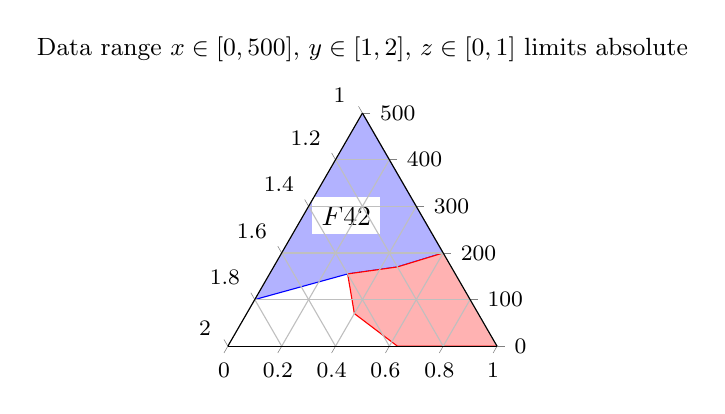
\begin{tikzpicture}
\begin{ternaryaxis}[
	ternary limits relative=false,
	xmax=500,ymin=1,ymax=2,
	title={Data range $x\in[0,500]$, 
		$y\in[1,2]$, $z\in[0,1]$ limits absolute},
	footnotesize, % just for the sake of demonstration...
	area style]
\addplot3 coordinates {
	(100,1.8,0)
	(155,1.4,0.29)
	(170,1.2,0.46)
	(200,1,0.6)
	(500,1,0)
};
\addplot3 coordinates {
	(200,1,0.6)
	(170,1.2,0.46)
	(155,1.4,0.29)
	(70,1.46,0.4)
	(0,1.37,0.63)
	(0,1,1)
};
\node[fill=white] 
	at (axis cs:280,1.28,0.16) {$F 42$};
\node[fill=white] 
	at (0.7,0.2) {$F 43$};
\end{ternaryaxis}
\end{tikzpicture}
\end{document}
